\section{Urban Data Layer (UDL)}
{{\footnotesize
\begin{description}[labelwidth=5em, labelsep=1em, leftmargin=*, align=left, itemsep=0.3em, parsep=0em]
  \item[date:] 2024-12-13
  \item[version:] TODO
  \item[last\_updated:] 2024-12
  \item[expired:] unknown
  \item[valid:] yes
  \item[valid\_date:] TODO
  \item[url:] \href{https://neurips.cc/virtual/2024/poster/97837}{https://neurips.cc/virtual/2024/poster/97837}
  \item[doi:] TODO
  \item[domain:] Urban Computing; Data Engineering
  \item[focus:] Unified data pipeline for multi-modal urban science research
  \item[keywords:]
    - data pipeline
    - urban science
    - multi-modal
    - benchmark
  \item[summary:] UrbanDataLayer standardizes heterogeneous urban data formats and provides pipelines for tasks like air quality prediction and land-use classification, enabling the rapid creation of multi-modal urban benchmarks :contentReference[oaicite:5]\{index=5\}.

  \item[licensing:] TODO
  \item[task\_types:]
    - Prediction
    - Classification
  \item[ai\_capability\_measured:]
    - Multi-modal urban inference
    - standardization
  \item[metrics:]
    - Task-specific accuracy or RMSE
  \item[models:]
    - Baseline regression/classification pipelines
  \item[ml\_motif:]
    - Data engineering
  \item[type:] Framework
  \item[ml\_task:]
    - Prediction, classification
  \item[solutions:] TODO
  \item[notes:] Source code available on GitHub (SJTU-CILAB/udl); promotes reusable urban-science foundation models :contentReference[oaicite:6]\{index=6\}.

  \item[contact.name:] Yiheng Wang
  \item[contact.email:] unknown
  \item[results.links.name:] ChatGPT LLM
  \item[fair.reproducible:] Yes
  \item[fair.benchmark\_ready:] Yes
  \item[ratings.software.rating:] 0
  \item[ratings.software.reason:] Not analyzed.

  \item[ratings.specification.rating:] 9.0
  \item[ratings.specification.reason:] Three tasks (de novo generation, retrieval, simulation) are clearly defined for MS/MS molecule discovery.

  \item[ratings.dataset.rating:] 10.0
  \item[ratings.dataset.reason:] Over 1 million spectra with structure annotations; dataset is open-source and well-documented.

  \item[ratings.metrics.rating:] 9.0
  \item[ratings.metrics.reason:] Task-appropriate metrics (structure accuracy, precision, MSE) are specified and used consistently.

  \item[ratings.reference\_solution.rating:] 8.0
  \item[ratings.reference\_solution.reason:] Baseline models are available (graph-based and retrieval), though not exhaustive.

  \item[ratings.documentation.rating:] 9.0
  \item[ratings.documentation.reason:] GitHub repo and poster provide code and reproducibility guidance.

  \item[id:] urban\_data\_layer\_udl
  \item[Citations:] \cite{neurips2024_0db7f135}
  \item[Ratings:]
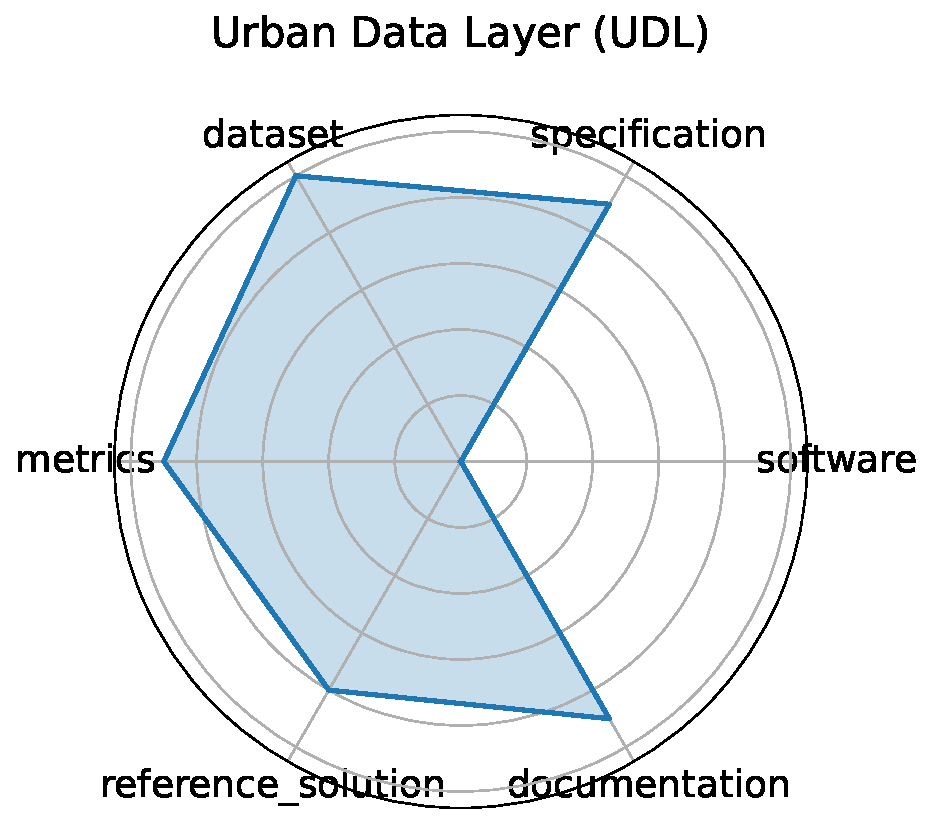
\includegraphics[width=0.2\textwidth]{urban_data_layer_udl_radar.pdf}
\end{description}
}}
\clearpage